\documentclass{beamer}

\usetheme{NapiziaMeeting}
%\usetheme{NapiziaMeetingLite}

\usepackage{graphicx}

%%  %%  %%  %%  %%  %%  %%  %%  %%  %%  %%  %%  %%  %%  %%  %%  %%  %%  %%  %%

\title{Sicilian Translator}
%% \author{Eryk Wdowiak}
\author{\texorpdfstring{Eryk Wdowiak\newline\href{eryk@wdowiak.me}{\texttt{eryk@wdowiak.me}}}{Eryk Wdowiak}}
\institute{Arba Sicula}
\date{27 Sep 2021}

%\usepackage{hyperref}
\hypersetup{
  %% bookmarks,
  %% bookmarksopen,
  colorlinks=true,
  linkcolor=blue,
  %% citecolor=black,
  %% filecolor=black,
  urlcolor=blue,
  bookmarksnumbered=false,
  pdftitle = {Sicilian Translator},
  pdfauthor = {Eryk Wdowiak},
  %% pdfsubject = {The Quarterly Review of Quarterly Reviews (2021), vol. xx, p. yy-zz},
  pdfkeywords = {Sicilian language, neural machine translation},
}

%%  %%  %%  %%  %%  %%  %%  %%  %%  %%  %%  %%  %%  %%  %%  %%  %%  %%  %%  %%

\begin{document}

%%  %%  %%  %%  %%  %%  %%  %%  %%  %%

\begin{frame}
  \titlepage
\end{frame}

%%  %%  %%  %%  %%  %%  %%  %%  %%  %%

\begin{frame}
  \frametitle{Why don't we have a Sicilian Translator?}
  \vspace{-1.0em}
  \begin{itemize}
    %%
  \item \href{https://translate.google.com/}{Google Translate} doesn't translate the Sicilian language.
    %%
  \item Nor does \href{https://www.bing.com/translator/}{Bing Translator},
    \href{https://translate.yandex.com/}{Yandex Translate} or
    \href{https://www.deepl.com/translator}{DeepL Translator}.
    %%
    \vspace{1em}
    \item Why not?  What are we going to do about it?
    %%
  \end{itemize} 
\end{frame}

%%  %%  %%  %%  %%  %%  %%  %%  %%  %%

\begin{frame}
  \frametitle{What is the Sicilian Language?}
  \vspace{-1.0em}
  \begin{itemize}
    %%
  \item The Sicilian School of Poets at the imperial court of Frederick II:
    \begin{itemize}
    \item created the first literary standard in Italy (13th century)
    \item inspired Dante, the ``father of the Italian language''
    \end{itemize}
    %%
  \vspace{0.65em}
  \item \underline{Sicilian emerged as a literary language before Italian}.
    %%   
  \vspace{1em}
  \item The people of Sicily, Calabria and Puglia speak it everyday.
    \begin{itemize}
    \item They speak Italian at work.
    \item But at home -- with family and friends -- they speak Sicilian.
    \item More precisely, their own dialect of the language.
    \end{itemize}
    %%
  \vspace{0.65em}
  \item And Sicilian is a language spoken here in Brooklyn, NY.
    %%   
  \end{itemize} 
\end{frame}

%%  %%  %%  %%  %%  %%  %%  %%  %%  %%

\begin{frame}
  \frametitle{So why don't we have a Sicilian Translator?}
  \vspace{-1.0em}
  \begin{itemize}
    %%
  \item No one had assembled the parallel text to train a translator.
    %%
    \vspace{1em}
    \item There's plenty!  For over 40 years, \href{http://www.arbasicula.org/}{Arba Sicula} has been:
      %% promoting Sicilian language and culture by:
    \begin{itemize}
    \item organizing poetry recitals, concerts, cultural events and tours of Sicily
    \item publishing books on Sicilian language, literature, history, cuisine, fiction, ...
    \item translating Sicilian poetry and prose
    \item publishing a bilingual journal, \textit{Arba Sicula}.
    \end{itemize}
    %%
  \vspace{1em}
  \item So we assembled the parallel text.
    %%
  \end{itemize} 
\end{frame}

%%  %%  %%  %%  %%  %%  %%  %%  %%  %%

\begin{frame}
  \frametitle{Sicilian Translator}
  \vspace{-1.0em}
  \href{https://translate.napizia.com}{%
    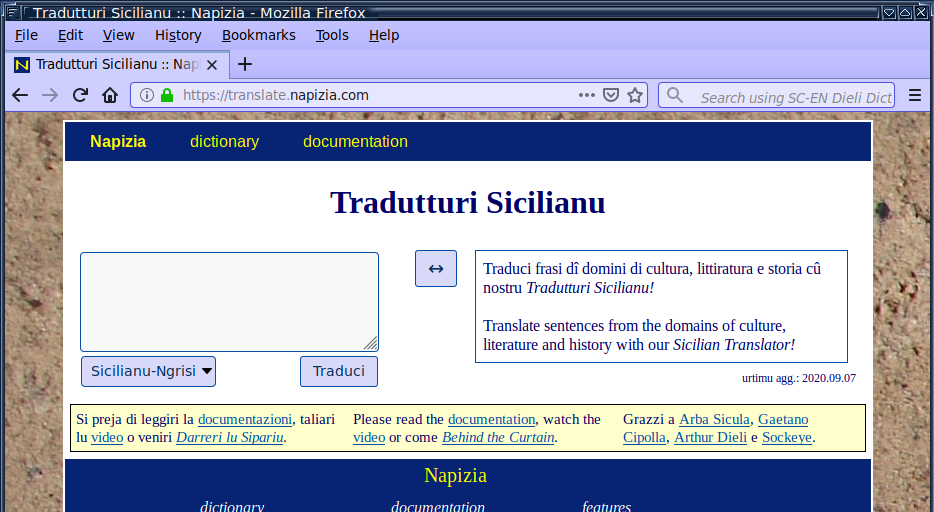
\includegraphics[width=\textwidth]{images/browser-white-box_v1.png}
  }
  \vspace{-1.0em}
  \hspace{-7.0pt}
  \footnotesize{\href{https://translate.napizia.com}{\texttt{https://translate.napizia.com}}}
\end{frame}

%%  %%  %%  %%  %%  %%  %%  %%  %%  %%

\begin{frame}
  \frametitle{How did we do it?}
  \vspace{-1.0em}
  \begin{itemize}
    %%
  \item We did \textbf{NOT} start with data collection.
    %%
  \vspace{1em}
  \item We started by collecting the rules of Sicilian vocabulary and grammar.
    \begin{itemize}
    \item Arthur Dieli's \href{http://www.dieli.net/SicilyPage/SicilianLanguage/Vocabulary.html}{\textit{Sicilian Vocabulary}}
    \item Kirk Bonner's \href{http://www.arbasicula.org/LegasOnlineStore.html\#!/28-An-Introduction-to-Sicilian-Grammar-by-J-K-Kirk-Bonner-Edited-by-Gaetano-Cipolla/p/82865123/category=0}{\textit{Introduction to Sicilian Grammar}} (2001)
    \item Gaetano Cipolla's \href{http://www.arbasicula.org/LegasOnlineStore.html\#!/26-Learn-Sicilian-Mparamu-lu-sicilianu-by-Gaetano-Cipolla/p/82865121/category=0}{\textit{Mparamu lu sicilianu}} (2013)
    \end{itemize}
    %%
    \vspace{1em}
    \item And we created the \href{https://www.napizia.com/cgi-bin/cchiu-da-palora.pl}{\textit{Chiù dâ Palora}}
  (\textit{More About the Word}) dictionary.
    \begin{itemize}
    \item vocabulary annotated with grammar, proverbs, poetry, prose and examples
    \item provides a reference for standardizing Sicilian language text
    \end{itemize}
  \end{itemize}
\end{frame}

%%  %%  %%  %%  %%  %%  %%  %%  %%  %%

\begin{frame}
  \frametitle{More About the Word}
  \vspace{-1.25em}
  \begin{center}
  \href{https://www.napizia.com/cgi-bin/cchiu-da-palora.pl}{%%
    %% 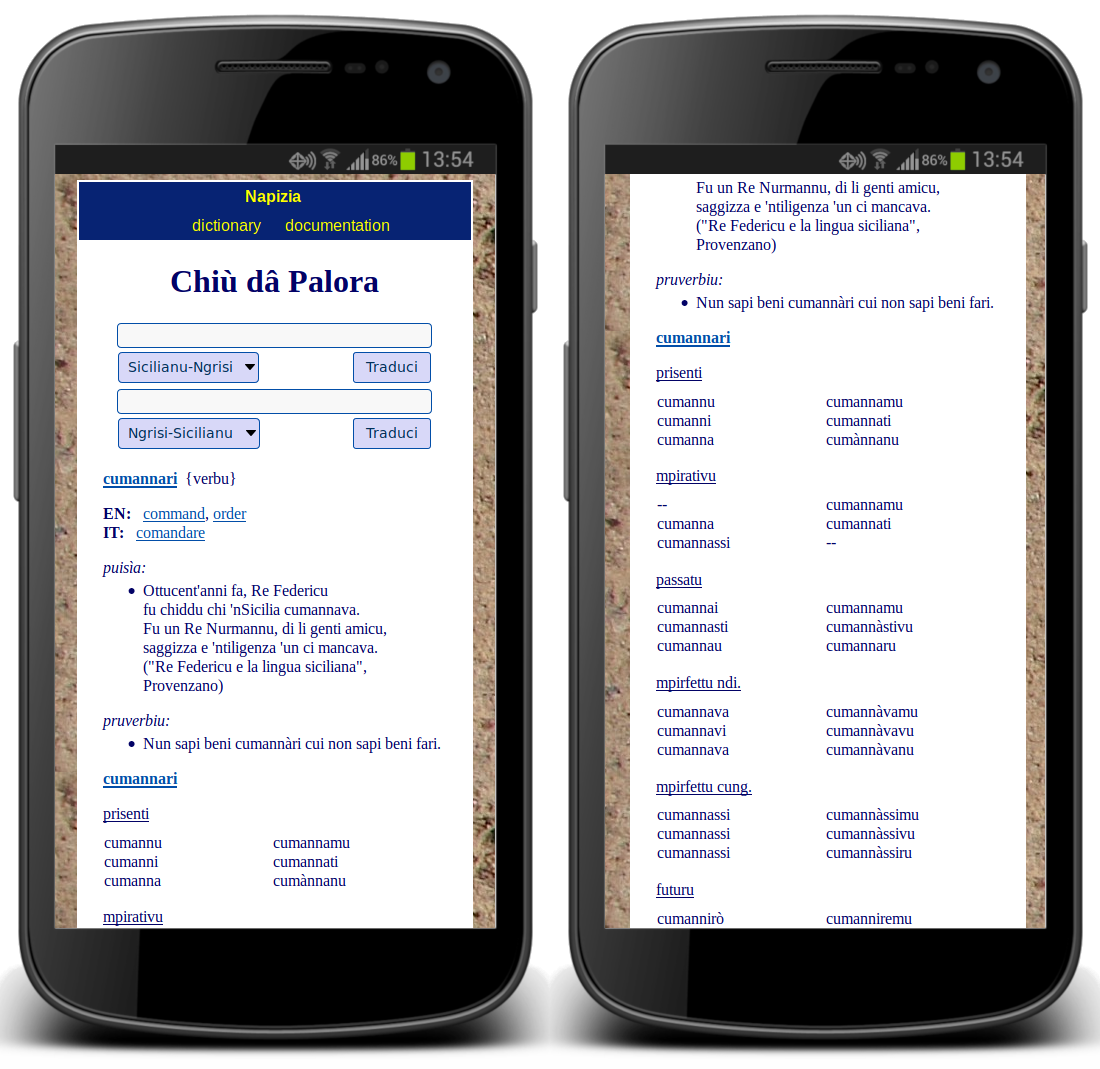
\includegraphics[height=0.795\textheight]{images/cdp_cumannari_v2.png}
    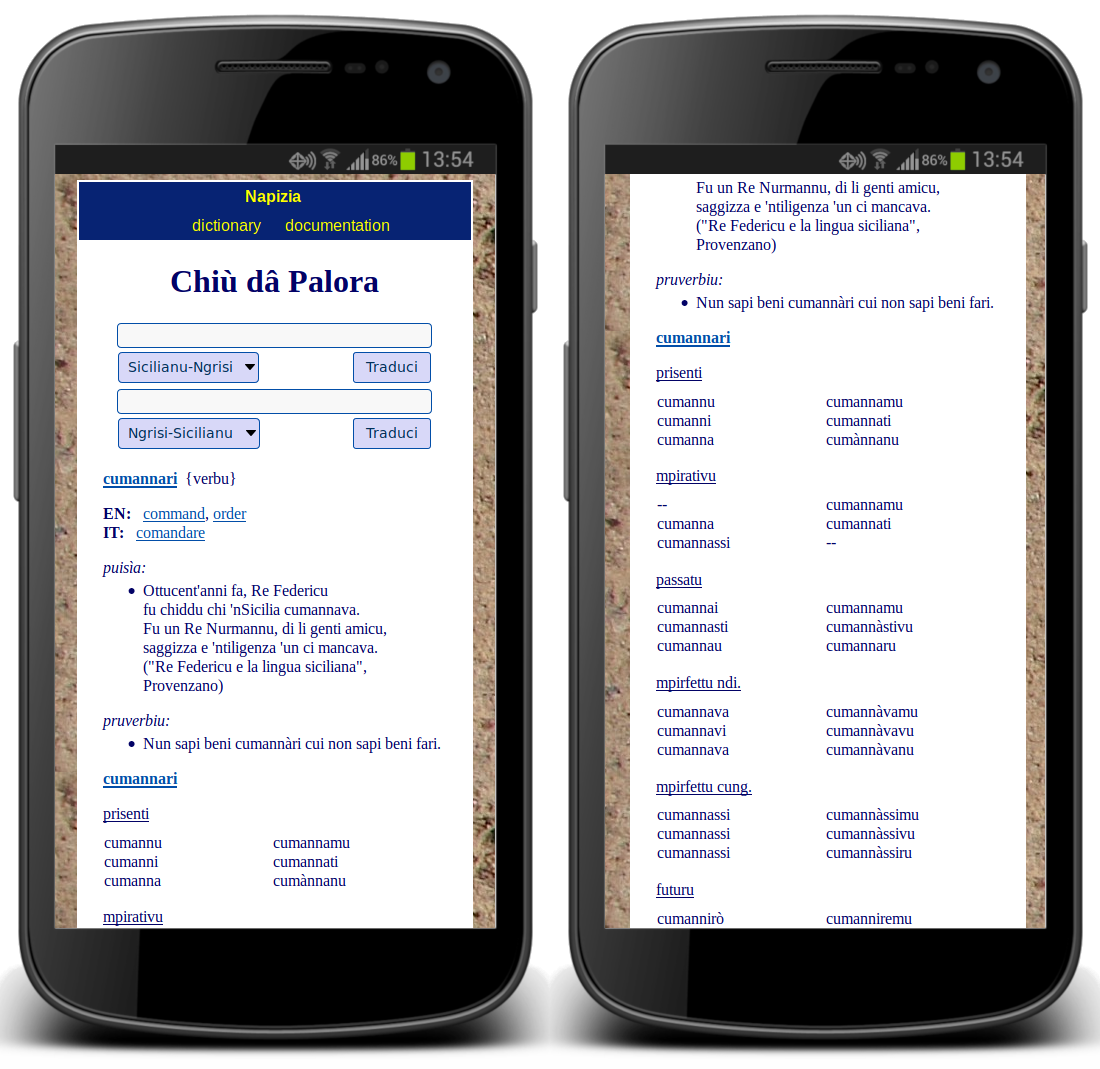
\includegraphics[height=0.755\textheight]{images/cdp_cumannari_v2.png}
  }
  \end{center}
  \vspace{-0.80em}
  \footnotesize{\href{https://www.napizia.com/cgi-bin/cchiu-da-palora.pl}{\texttt{https://www.napizia.com/cgi-bin/cchiu-da-palora.pl}}}
\end{frame}


%%  %%  %%  %%  %%  %%  %%  %%  %%  %%

\begin{frame}
  \frametitle{Then We Began Collecting Data}
  \vspace{-1.0em}
  \begin{itemize}
  \item Sources of parallel text:
    \begin{itemize}
    \item the bilingual literary journal \href{https://www.arbasicula.org/}{\textit{Arba Sicula}}
    \item \href{http://www.dieli.net/}{A.~Dieli}'s translations of Sicilian poetry, proverbs and \href{https://en.wikipedia.org/wiki/Giuseppe_Pitr\%C3\%A8}{G.~Pitrè}'s \href{https://scn.wikipedia.org/wiki/F\%C3\%A0uli,_nueddi_e_cunti_pupulari_siciliani}{\textit{Folk Tales}}
    \item examples from G.~Cipolla's \href{http://www.arbasicula.org/LegasOnlineStore.html\#!/26-Learn-Sicilian-Mparamu-lu-sicilianu-by-Gaetano-Cipolla/p/82865121/category=0}{\textit{Mparamu}} and K.~Bonner's \href{http://www.arbasicula.org/LegasOnlineStore.html\#!/28-An-Introduction-to-Sicilian-Grammar-by-J-K-Kirk-Bonner-Edited-by-Gaetano-Cipolla/p/82865123/category=0}{\textit{Introduction}}
   \end{itemize}
  %% \item Textbook examples greatly improved translation quality. (See below).
  \vspace{0.5em}
  \item Data Preparation
    \begin{itemize}
    \item Selected Sicilian language text that could be edited to Standard Sicilian.
    \item Used \href{https://github.com/danielvarga/hunalign}{\textit{hunalign}} to identify translated sentence pairs.
    \item Manually edited the text (both languages) for quality and standardization.
    \end{itemize}
  \vspace{0.5em}
  \item Our parallel corpus (so far):
    \begin{itemize}
    \item 12,357 lines of bilingual text -- 237,456 Sicilian words, 236,568 English words
    \item 4,660 lines of trilingual textbook exercises -- Sicilian, English and Italian
    \item 121 hand-selected lines for validation {\small{(in all three languages)}}
    \item the Italian-English subset of \href{https://farkastranslations.com/bilingual_books.php}{Farkas' \textit{Books}}
    \end{itemize}
  \end{itemize} 
\end{frame}

%%  %%  %%  %%  %%  %%  %%  %%  %%  %%

\begin{frame}
  \frametitle{And We Began Modeling}
  \vspace{-1.0em}
  \begin{itemize}
  \item We trained our translation models with \href{https://awslabs.github.io/sockeye/}{Sockeye}.
  \vspace{0.25em}
  \item Adding parallel text always improves translation quality more than adjusting hyperparameters.
  \vspace{0.25em}
  \item But some ways of training a model are better than others.
  \vspace{0.25em}
  \item We avoid overfitting by training:
    \begin{itemize}
    \item a self-attentional Transformer model \href{https://arxiv.org/abs/1706.03762}{(Vaswani et al., 2017)}%%,
      %% which directly models the relationships between words in a pair of sentences.
    \item a smaller network with fewer layers \href{https://arxiv.org/abs/1905.11901}{(Sennrich and Zhang, 2019)}
    \item with small subword vocabularies \href{https://arxiv.org/abs/1508.07909}{(Sennrich, Haddow and Birch, 2016)}
    \item with high-dropout parameters \href{http://jmlr.org/papers/v15/srivastava14a.html}{(Srivastava et al., 2014)}
    \end{itemize}
  \vspace{0.25em}
  \item Large empirical improvements when we added theoretical knowledge:
    \begin{itemize}
    \item by pushing the subword distribution toward textbook desinences
    \item by using textbook examples to give structure to the sequences
    \end{itemize}
  \end{itemize}
\end{frame}

%%  %%  %%  %%  %%  %%  %%  %%  %%  %%

\begin{frame}
  \frametitle{Evaluation Metrics}
  \vspace{-1.0em}
  \begin{itemize}
    %%
  \item BLEU score -- measure of translation quality
    %%
    \begin{itemize}
    %% \item Precision-based measure that compares candidate and reference translations.
    \item Higher when sequences of words in the candidate translation match sequences in the reference translation.
    \item Highly correlated with human judgements of translation quality.
    \end{itemize} 
    %%
    \vspace{0.5em}
  \item What's a good score?
    \begin{itemize}
    \item In theory, BLEU score ranges from 0 to 100.
    \item In practice, there are many ways to translate a sentence.
    \item Scores reported by \href{https://arxiv.org/abs/1706.03762}{Vaswani et al. (2017)}:
      \begin{itemize} 
      \item 41.8 on English-to-French translation
      \item 28.4 on English-to-German translation
      \end{itemize} 
    \end{itemize} 
    %%
    \vspace{0.5em}
  \item Our \href{https://translate.napizia.com}{\textit{Tradutturi Sicilianu}} achieved BLEU scores of:
    %% 
    \begin{itemize}
    \item 35.0 on English-to-Sicilian,~  36.8 on Sicilian-to-English
    \item 36.5 on Italian-to-Sicilian,~~ 30.9 on Sicilian-to-Italian
    \end{itemize} 
    %%
  \end{itemize} 
\end{frame}

%%  %%  %%  %%  %%  %%  %%  %%  %%  %%

\begin{frame}
  \frametitle{Comparing Models}
  \vspace{-1.0em}
  \begin{itemize}
  \item Translation quality improves with parallel text.  As our dataset grew
    from 120,000 to 270,000 words, our BLEU scores increased:
    \begin{itemize}
    \item from 11.4 to 25.1 on English-to-Sicilian translation
    \item from 12.9 to 29.1 on Sicilian-to-English translation
    \end{itemize}
  \vspace{0.5em}
  \item Within a given dataset, pushing the subword distribution toward textbook desinences increased BLEU scores:
    \begin{itemize}
    \item from 20.3 to 22.4 on English-to-Sicilian translation
    \item from 21.4 to 24.1 on Sicilian-to-English translation
    \end{itemize}
  \vspace{0.5em}
  \item We also observed larger increases in BLEU scores when we added parallel text from 
    textbook examples than from other sources.
    \begin{itemize}
    \item We did not conduct any formal tests to confirm this observation.
    \item With our eyes, we could see the structure that textbook examples added.
    \end{itemize}
  \end{itemize} 
\end{frame}

%%  %%  %%  %%  %%  %%  %%  %%  %%  %%

\begin{frame}
  \frametitle{Multilingual Translation}
  \vspace{-1.0em}
  \begin{itemize}
  %% \item We still have more issues of \href{https://www.arbasicula.org/}{\textit{Arba Sicula}} to extract text from.
  %% \item So we'll add more parallel text and further increase translation quality.
  \item To further improve translation quality, we added the Italian-English subset of
    \href{https://farkastranslations.com/bilingual_books.php}{Farkas' \textit{Books}}
    (from the \href{http://opus.nlpl.eu/}{OPUS project}) to our dataset.
    \vspace{0.35em}
  \item To enable multilingual translation, we added a directional token -- ex. \texttt{<2it>} (``to Italian'') -- to the
    source sequence \href{https://arxiv.org/abs/1611.04558}{(Johnson et al., 2016)}.
    \vspace{0.35em}
  \item And we trained a larger model \href{https://arxiv.org/abs/1907.05019}{(Arivazhagan et al., 2019)}
    with a ``bridging strategy'' \href{https://arxiv.org/abs/2010.11125}{(Fan et al., 2020)}.
    \vspace{0.35em}
  \item This further improved translation quality. Our BLEU scores increased:
    \begin{itemize}
    \item from 25.1 to 35.0 on English-to-Sicilian %% translation
    \item from 29.1 to 36.8 on Sicilian-to-English %% translation
    \end{itemize}
    \vspace{0.25em}
  \item And it yielded good translation quality between Sicilian and Italian:
    \begin{itemize}
    \item 36.5 on Italian-to-Sicilian %% translation
    \item 30.9 on Sicilian-to-Italian %% translation
    \end{itemize}    
  %% 
  %%  \vspace{1em}
  %%\item We may also use the Sicilian text to train word embeddings and create lists of context similar words for our dictionary,
  %%  \href{https://www.napizia.com/cgi-bin/cchiu-da-palora.pl}{\textit{Chiù dâ Palora}}.
  %%  \vspace{1em}
  %%  \item And we'll add more poetry, proverbs and prose to the dictionary too.
  \end{itemize}
\end{frame}

%%  %%  %%  %%  %%  %%  %%  %%  %%  %%

\begin{frame}
  \frametitle{Come to Napizia!}
  \vspace{-1.0em}
  \begin{itemize}
  \item So come to \href{https://www.napizia.com/index.shtml}{\textit{Napizia}} and try our
    \href{https://translate.napizia.com}{\textit{Tradutturi Sicilianu}}\textit{:}
    \begin{itemize}
    \item \footnotesize{\href{https://translate.napizia.com}{\texttt{https://translate.napizia.com}}}
    \end{itemize}
    \vspace{0.65em}
  \item To see how it works ``behind the curtain,'' come
    \href{https://translate.napizia.com/cgi-bin/darreri.pl}{\textit{Darreri lu Sipariu}}\textit{:}
    \begin{itemize}
    \item \footnotesize{\href{https://translate.napizia.com/cgi-bin/darreri.pl}{\texttt{https://translate.napizia.com/cgi-bin/darreri.pl}}}
    \end{itemize}
    \vspace{0.65em}
  %% \item Try our \href{https://www.doviak.net/pages/ml-sicilian/ml-scn_p05.shtml}{``Recipe for Low-Resource NMT''}
  \item Read our \href{https://www.doviak.net/pages/ml-sicilian/}{``Introduction to Sicilian NLP''}
    \begin{itemize}
    %% \item \footnotesize{\href{https://www.doviak.net/pages/ml-sicilian/ml-scn_p05.shtml}{\texttt{https://www.doviak.net/pages/ml-sicilian/ml-scn\_p05.shtml}}}
    \item \footnotesize{\href{https://www.doviak.net/pages/ml-sicilian/}{\texttt{https://www.doviak.net/pages/ml-sicilian/}}}
    \end{itemize}
    \vspace{0.65em}
  \item And check out our \href{https://github.com/ewdowiak/Sicilian_Translator}{\texttt{Sicilian\_Translator}} repository at Github:
    \begin{itemize}
    \item \footnotesize{\href{https://github.com/ewdowiak/Sicilian_Translator}{\texttt{https://github.com/ewdowiak/Sicilian\_Translator}}}
    \end{itemize}
    \vspace{0.65em}
  \item We hope you'll join us. %% \textit{Grazzi!}
  \end{itemize}
\end{frame}

%% \item \href{https://www.napizia.com/pages/sicilian/translator.shtml}{Sicilian Translator} at Napizia
%% \item \href{https://www.doviak.net/pages/ml-sicilian/index.shtml}{Introduction to Sicilian NLP}

%%  %%  %%  %%  %%  %%  %%  %%  %%  %%

\begin{frame}
  \frametitle{Acknowledgements}
  \vspace{-1.0em}
  \begin{itemize}
  \item Thank you to \href{https://www.arbasicula.org/}{Arba Sicula}, 
    \href{https://en.wikipedia.org/wiki/Gaetano_Cipolla}{Gaetano Cipolla} and 
    \href{http://www.dieli.net/}{Arthur Dieli}:
    \vspace{0.20em}
    \begin{itemize}
    \item for developing the resources that made this project possible
      \vspace{0.20em}
    \item for their support and encouragement
      \vspace{0.20em}
    \item for sponsoring and developing Sicilian language and culture
    \end{itemize}
    \vspace{0.35em}
  \item \textit{Grazzi!}
  \end{itemize} 
\end{frame}

%%  %%  %%  %%  %%  %%  %%  %%  %%  %%

\end{document}

%%  %%  %%  %%  %%  %%  %%  %%  %%  %%
% %%  %%  %%  %%  %%  %%  %%  %%  %%
%%  %%  %%  %%  %%  %%  %%  %%  %%  %%

%% \begin{frame}
%%   \frametitle{frame title}
%%   \vspace{-1.0em}
%%   \begin{itemize}
%%   \item text
%%   \item text
%%   \end{itemize} 
%% \end{frame}

%%  %%  %%  %%  %%  %%  %%  %%  %%  %%

%% \hspace{-1pt}
%% 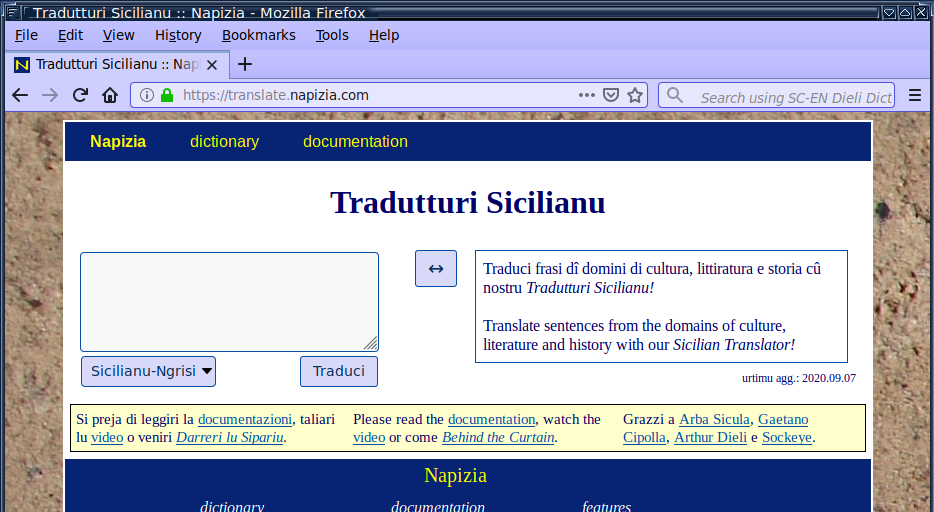
\includegraphics[
%%   %% trim={"left"}{"bottom"}{"right"}{"top"}
%%   trim={0.0in} {0.0in} {0.0in} {0.0in},
%%   clip=true]{images/browser-white-box_v1.png}

%%  %%  %%  %%  %%  %%  %%  %%  %%  %%
